\documentclass{article}
\usepackage{graphicx}  % for including figures
\usepackage{amsmath,amsthm,amssymb,hyperref,nicematrix, tikz}
\usepackage{arydshln}
\usepackage{mathrsfs}
\usepackage{mathtools}
\usepackage{enumitem}
\usepackage{tikzsymbols}
\usepackage{float} % For using H in figure position.
\usepackage{bm}
\usepackage[numbered,framed]{matlab-prettifier}
\usepackage{gensymb}
\usepackage{pgffor}
\usepackage{booktabs} % Uses \toprule, midrule, etc. for tables.

\newcommand\independent{\protect\mathpalette{\protect\independenT}{\perp}}

\newcommand{\blue}{\color{blue}}

\NiceMatrixOptions
  {
    custom-line = 
     {
       letter=I, 
       command=hdashedline, 
       tikz=densely dashed,
       width=\pgflinewidth
     },
     cell-space-limits = 1pt
  }

\def\independenT#1#2{\mathrel{\rlap{$#1#2$}\mkern2mu{#1#2}}}
\lstset{style=Matlab-editor}
\newcommand{\R}{\mathbb{R}}
\newcommand{\bigrho}{\raisebox{-.15\baselineskip}{\Large\ensuremath{\rho}}} 

% ------------------------------------------ %
%                   START HERE               %
% ------------------------------------------ %

\begin{document}

\title{Applied Multivariate Statistical Analysis Solutions}
\author{Nathan Crouse}
\maketitle

\tableofcontents

\section{Chapter 1}

% \section{Chapter 2}
% \foreach \n in {1,...,42}{
%     \subsection{}
%     \input{chapter-2/question-2-\n}
% }
% \newpage
% \section{Chapter 3}
% \foreach \n in {1,...,20}{
%     \subsection{}
%     \input{chapter-3/question-3-\n}
% }
% \newpage
% \section{Chapter 4}
% \foreach \n in {1,...,41}{
%     \subsection{}
%     \input{chapter-4/question-4-\n}
% }

%Consider a bivariate normal distribution with $\mu_{1} = 1$, $\mu_{2} = 3$, $\sigma_{11} = 2$, $\sigma_{22} = 1$ and $\rho_{12} = -0.8$.
\begin{enumerate}[label=(\alph*)]
    \item Write out the bivariate normal density.
    For
    \[
        \textbf{x}
        =
        \begin{bNiceArray}{c}
            X_1 \\
            X_2
        \end{bNiceArray},
        \hspace{0.2in}
        \bm{\mu}
        =
        \begin{bNiceArray}{c}
            \mu_1 \\
            \mu_2
        \end{bNiceArray}
        =
        \begin{bNiceArray}{c}
            1 \\
            3
        \end{bNiceArray},
        \hspace{0.2in}
    \]
    \[
        \bm{\Sigma}
        =
        \begin{bNiceArray}{cc}
            \sigma_{11} & \sqrt{\sigma_{11}}\sqrt{\sigma_{22}}\rho_{12} \\
            \sqrt{\sigma_{11}}\sqrt{\sigma_{22}}\rho_{12} & \sigma_{22}
        \end{bNiceArray}
        =
        \begin{bNiceArray}{cc}
            2 & -0.80\sqrt{2} \\
            -0.80\sqrt{2} & 1
        \end{bNiceArray}
    \]
    \[
        f(\textbf{x} \big| \bm{\mu},\bm{\Sigma})
        =
        \frac{1}{{(2\pi)}^{p/2}{\left|\bm{\Sigma}\right|}^{1/2}}
        {e}^{\frac{-1}{2}{(\textbf{x} - \bm{\mu})}^{\prime}\bm{\Sigma}(\textbf{x} - \bm{\mu})}
        =
    \]
    \begin{multline*}
        =
        \frac{1}{{(2\pi)}^{2/2}\sqrt{\sigma_{11}\sigma_{22}(1-\rho_{12}^2)}}
        \exp
        \Bigg{\{}
            \frac{-1}{2(1-\rho_{12}^2)}
            \Bigg{[}
                {\left(\frac{x_1 - \mu_1}{\sqrt{\sigma_{11}}}\right)}^{2}
                +
                {\left(\frac{x_2 - \mu_2}{\sqrt{\sigma_{22}}}\right)}^{2} \\
                -
                2\rho_{12}
                \left(\frac{x_1 - \mu_1}{\sqrt{\sigma_{11}}}\right)
                \left(\frac{x_2 - \mu_2}{\sqrt{\sigma_{22}}}\right)
            \Bigg{]}
        \Bigg{\}}
        =
    \end{multline*}
    \begin{multline*}
        =
        \frac{1}{{(2\pi)}^{2/2}\sqrt{2(1-0.64)}}
        \exp
        \Bigg{\{}
            \frac{-1}{2(1-0.64)}
            \Bigg{[}
                {\left(\frac{x_1 - 1}{\sqrt{2}}\right)}^{2}
                +
                {\left(\frac{x_2 - 3}{\sqrt{1}}\right)}^{2} \\
                +
                2(0.80)
                \left(\frac{x_1 - 1}{\sqrt{2}}\right)
                \left(\frac{x_2 - 3}{\sqrt{1}}\right)
            \Bigg{]}
        \Bigg{\}}
        =
    \end{multline*}
    \begin{multline*}
        =
        \frac{1}{1.2\pi\sqrt{2}}
        \exp
        \Bigg{\{}
            \frac{-1}{0.72}
            \Bigg{[}
                {\left(\frac{x_1 - 1}{\sqrt{2}}\right)}^{2}
                +
                {\left(x_2 - 3\right)}^{2} \\
                +
                1.6
                \left(\frac{x_1 - 1}{\sqrt{2}}\right)
                \left(x_2 - 3\right)
            \Bigg{]}
        \Bigg{\}}
    \end{multline*}
    \item Write out the squared statistical distance expression ${(\textbf{x} - \bm{\mu})}^{\prime}\bm{\Sigma}^{-1}{(\textbf{x} - \bm{\mu})}$ as a quadratic
    function of $x_1$ and $x_2$.
    \par
    This is most of what's inside the exponent.
    \[
        {(\textbf{x} - \bm{\mu})}^{\prime}\bm{\Sigma}^{-1}{(\textbf{x} - \bm{\mu})}
        =
    \]
    \[
        =
        \frac{1}{1-\rho_{12}^2}
        \Bigg{[}
            {\left(\frac{x_1 - \mu_1}{\sqrt{\sigma_{11}}}\right)}^{2}
            +
            {\left(\frac{x_2 - \mu_2}{\sqrt{\sigma_{22}}}\right)}^{2} \\
            -
            2\rho_{12}
            \left(\frac{x_1 - \mu_1}{\sqrt{\sigma_{11}}}\right)
            \left(\frac{x_2 - \mu_2}{\sqrt{\sigma_{22}}}\right)
        \Bigg{]}
        =
    \]
    \[
        =
        \frac{1}{0.36}
        \Bigg{[}
            {\left(\frac{x_1 - 1}{\sqrt{2}}\right)}^{2}
            +
            {\left(\frac{x_2 - 3}{1}\right)}^{2} \\
            +
            1.6
            \left(\frac{x_1 - 1}{\sqrt{2}}\right)
            \left(x_2 - 3\right)
        \Bigg{]}
        =
    \]
    \[
        =
        \frac{1}{0.36}
        \Bigg{[}
            \frac{1}{2}
            ({x_1}^{2} - 2x_1 + 1)
            +
            ({x_2}^{2} - 6x_2 + 9)
            +
            \frac{1.6\sqrt{2}}{2}
            (x_1 x_2 -3x_1 - x_2 + 3)
        \Bigg{]}
        =
    \]
    \[
        =
        \frac{1}{0.36}
        \Bigg{[}
            \frac{1}{2}
            ({x_1}^{2} - 2x_1 + 1)
            +
            ({x_2}^{2} - 6x_2 + 9)
            +
            \frac{1.6\sqrt{2}}{2}
            (x_1 x_2 -3x_1 - x_2 + 3)
        \Bigg{]}
        =
    \]
    \[
        =
        \frac{25}{18}
        {x_1}^{2}
        +
        \frac{50}{18}
        {x_2}^{2}
        -
        \frac{5(5+12\sqrt{2})}{9}
        x_1
        -
        x_2
        \frac{10(15 + 2\sqrt{2})}{9}
        +
        \frac{20\sqrt{2}}{9}
        x_1
        x_2
        +
        \frac{5(95+24\sqrt{2})}{18}
        =
    \]
    \[
        =
        1.3889
        x_1^2
        +
        2.7778
        x_2^2
        -
        12.2059
        x_1
        -
        19.8094
        x_2
        +
        3.1427
        x_1 x_2
        +
        35.8170
    \]
\end{enumerate}
% Consider a bivariate normal distribution with $\mu_{1} = 0$, $\mu_{2} = 2$, $\sigma_{11} = 2$, $\sigma_{22} = 1$ and $\rho_{12} = 0.5$.
\begin{enumerate}[label=(\alph*)]
    \item Write out the bivariate normal density.
    For
    \[
        \textbf{x}
        =
        \begin{bNiceArray}{c}
            X_1 \\
            X_2
        \end{bNiceArray},
        \hspace{0.2in}
        \bm{\mu}
        =
        \begin{bNiceArray}{c}
            \mu_1 \\
            \mu_2
        \end{bNiceArray}
        =
        \begin{bNiceArray}{c}
            0 \\
            2
        \end{bNiceArray},
        \hspace{0.2in}
    \]
    \[
        \bm{\Sigma}
        =
        \begin{bNiceArray}{cc}
            \sigma_{11} & \sqrt{\sigma_{11}}\sqrt{\sigma_{22}}\rho_{12} \\
            \sqrt{\sigma_{11}}\sqrt{\sigma_{22}}\rho_{12} & \sigma_{22}
        \end{bNiceArray}
        =
        \begin{bNiceArray}{cc}
            2 & 0.50\sqrt{2} \\
            0.50\sqrt{2} & 1
        \end{bNiceArray}
    \]
    \[
        f(\textbf{x} \big| \bm{\mu},\bm{\Sigma})
        =
        \frac{1}{{(2\pi)}^{p/2}{\left|\bm{\Sigma}\right|}^{1/2}}
        {e}^{\frac{-1}{2}{(\textbf{x} - \bm{\mu})}^{\prime}\bm{\Sigma}(\textbf{x} - \bm{\mu})}
        =
    \]
    \begin{multline*}
        =
        \frac{1}{{(2\pi)}^{2/2}\sqrt{\sigma_{11}\sigma_{22}(1-\rho_{12}^2)}}
        \exp\Bigg{\{}\frac{-1}{2(1-\rho_{12}^2)}\Bigg{[}
        {\left(\frac{x_1 - \mu_1}{\sqrt{\sigma_{11}}}\right)}^{2}
        +
        {\left(\frac{x_2 - \mu_2}{\sqrt{\sigma_{22}}}\right)}^{2} \\
        -
        2\rho_{12}\left(\frac{x_1 - \mu_1}{\sqrt{\sigma_{11}}}\right)\left(\frac{x_2 - \mu_2}{\sqrt{\sigma_{22}}}\right)\Bigg{]}\Bigg{\}}
        =
    \end{multline*}
    \begin{multline*}
        =
        \frac{1}{{(2\pi)}^{2/2}\sqrt{2(1-0.25)}}
        \exp
        \Bigg{\{}
            \frac{-1}{2(1-0.25)}
            \Bigg{[}
                {\left(\frac{x_1 - 0}{\sqrt{2}}\right)}^{2}
                +
                {\left(\frac{x_2 - 2}{\sqrt{1}}\right)}^{2} \\
                -
                2(0.50)
                \left(\frac{x_1 - 0}{\sqrt{2}}\right)
                \left(\frac{x_2 - 2}{\sqrt{1}}\right)
            \Bigg{]}
        \Bigg{\}}
        =
    \end{multline*}
    \[
        =
        \frac{\sqrt{6}}{6\pi}
        \exp
        \Bigg{\{}
            \frac{-2}{3}
            \Bigg{[}
                {\frac{x_1^2}{2}}
                +
                {\left(x_2 - 2\right)}^{2}
                -
                \left(\frac{x_1}{\sqrt{2}}\right)
                \left(x_2 - 2\right)
            \Bigg{]}
        \Bigg{\}}
    \]
    \item Write out the squared statistical distance expression ${(\textbf{x} - \bm{\mu})}^{\prime}\bm{\Sigma}^{-1}{(\textbf{x} - \bm{\mu})}$ as a quadratic
    function of $x_1$ and $x_2$.
    \par
    This is most of what's inside the exponent.
    \[
        {(\textbf{x} - \bm{\mu})}^{\prime}\bm{\Sigma}^{-1}{(\textbf{x} - \bm{\mu})}
        =
    \]
    \[
        =
        \frac{1}{1-\rho_{12}^2}
        \Bigg{[}
            {\left(\frac{x_1 - \mu_1}{\sqrt{\sigma_{11}}}\right)}^{2}
            +
            {\left(\frac{x_2 - \mu_2}{\sqrt{\sigma_{22}}}\right)}^{2} \\
            -
            2\rho_{12}
            \left(\frac{x_1 - \mu_1}{\sqrt{\sigma_{11}}}\right)
            \left(\frac{x_2 - \mu_2}{\sqrt{\sigma_{22}}}\right)
        \Bigg{]}
        =
    \]
    \[
        =
        \frac{4}{3}
        \Bigg{[}
            \frac{1}{2}x_1^2
            +
            {\left(x_2 - 2\right)}^{2}
            +
            \left(\frac{x_1}{\sqrt{2}}\right)
            \left(x_2 - 2\right)
        \Bigg{]}
        =
    \]
    \[
        =
        \frac{4}{3}
        \Bigg{[}
            \frac{1}{2}x_1^2
            +
            {\left(x_2^2 - 4x_2 + 4\right)}
            +
            \frac{\sqrt{2}}{2}
            \left(x_1x_2 - 2x_1\right)
        \Bigg{]}
        =
    \]
    \[
        =
        \frac{2}{3}
        x_1^2
        +
        \frac{4}{3}
        x_2^2
        -
        \frac{4\sqrt{2}}{3}
        x_1
        -
        \frac{16}{3}
        x_2
        +
        \frac{2\sqrt{2}}{3}
        x_1 x_2
        -
        \frac{16}{3}
        =
    \]
    \[
        =
        0.6667
        x_1^2
        +
        1.3333
        x_2^2
        -
        1.8856
        x_1
        -
        5.3333
        x_2
        +
        0.9428
        x_1
        x_2
        +
        5.3333
    \]
    \item Determine (and sketch) the constant-density contour that contains 50\% of the probability.
    \newline
    \par
    First, find the eigenvalues.
    \[
        0
        =
        \left|
        \bm{\Sigma} - \lambda \textbf{I}
        \right|
        =
        \left|
            \begin{NiceArray}{cc}
                2 - \lambda & \sqrt{2}/2 \\
                \sqrt{2}/2  & 1 - \lambda
            \end{NiceArray}
        \right|
        =
        (2 - \lambda)(1 - \lambda) - \frac{2}{4}
        =
    \]
    \[
        =
        {\lambda}^2
        -
        3
        \lambda
        +
        2
        -
        \frac{1}{2}
        =
        {\lambda}^2
        -
        3
        \lambda
        +
        \frac{3}{2}
        =
        (\lambda - (3-\sqrt{3})/2)(\lambda - (3+\sqrt{3})/2)
    \]
    The eigenvalues are $(3\pm\sqrt{3})/2$.
    \newline
    \underline{$\lambda_1 = \frac{3 - \sqrt{3}}{2}$:}
    \[
        \bm{\Sigma}\textbf{x}_1 = \lambda_1\textbf{x}_1
        \Rightarrow
        \begin{bNiceArray}{cc}
            2 & \sqrt{2}/2 \\
            \sqrt{2}/2 & 1
        \end{bNiceArray}
        \begin{bNiceArray}{c}
            x_1 \\
            x_2
        \end{bNiceArray}
        =
        \begin{bNiceArray}{c}
            (3 - \sqrt{3})/2 x_1 \\
            (3 - \sqrt{3})/2 x_2
        \end{bNiceArray}
    \]
    \[
        \Rightarrow
        \begin{bNiceArray}{cc}
            (1+\sqrt{3})/2 & \sqrt{2}/2 \\
            \sqrt{2}/2 & (-1+\sqrt{3})/2
        \end{bNiceArray}
        \begin{bNiceArray}{c}
            x_1 \\
            x_2
        \end{bNiceArray}
        =
        \begin{bNiceArray}{c}
            0 \\
            0
        \end{bNiceArray}
    \]
    \[
        \Rightarrow
        \begin{bNiceArray}{cc}
            (1+\sqrt{3})/2 & \sqrt{2}/2 \\
            \sqrt{2}/2 & (-1+\sqrt{3})/2
        \end{bNiceArray}
        \overset{\text{Row 2} - \left(\frac{2}{1 + \sqrt{3}}\right)\frac{\sqrt{2}}{2}\text{Row 1}}{\longrightarrow}
        \begin{bNiceArray}{cc}
            (1+\sqrt{3})/2 &  \\
            0 & 0
        \end{bNiceArray}
    \]
\[
    \frac{(1+\sqrt{3})}{2} x_1 = -\frac{\sqrt{2}}{2} x_2
    \Rightarrow
    x_1 = - \frac{\sqrt{2}}{(1+\sqrt{3})} x_2
\]
\[
    \textbf{x}_1
    =
    \begin{bNiceArray}{c}
        - \frac{\sqrt{2}}{(1+\sqrt{3})} \\
        1
    \end{bNiceArray}
\]
\[
    \left\|
    \textbf{x}_1
    \right\|
    =
    \sqrt{
        {\left(- \frac{\sqrt{2}}{(1+\sqrt{3})}\right)}^{2}
        +
        1^2
    }
    =
    \sqrt{
        \frac{2 + (4 + 2\sqrt{3})}{{(1+\sqrt{3})}^{2}}
    }
    =
    \frac{\sqrt{2(3 + \sqrt{3})}}{(1+\sqrt{3})}
\]
\[
    \textbf{e}_1
    =
    \frac{\textbf{x}_1}{
        \left\|
            \textbf{x}_1
        \right\|
    }
    =
    \frac{(1+\sqrt{3})}{\sqrt{2(3 + \sqrt{3})}}
    \begin{bNiceArray}{c}
        - \frac{\sqrt{2}}{(1+\sqrt{3})} \\
        1
    \end{bNiceArray}
    =
    \begin{bNiceArray}{c}
        - \frac{1}{\sqrt{3 + \sqrt{3}}} \frac{\sqrt{3 - \sqrt{3}}}{\sqrt{3 - \sqrt{3}}} \\
        \frac{1+\sqrt{3}}{\sqrt{2(3 + \sqrt{3})}} \frac{\sqrt{3 - \sqrt{3}}}{\sqrt{3 - \sqrt{3}}}
    \end{bNiceArray}
    =
\]
\[
    =
    \begin{bNiceArray}{c}
        - \frac{\sqrt{3 - \sqrt{3}}}{\sqrt{6}} \frac{\sqrt{6}}{\sqrt{6}} \\
        \frac{\sqrt{2(3 + \sqrt{3})}}{\sqrt{12}} \frac{\sqrt{6}}{\sqrt{6}}
    \end{bNiceArray}
    =
    \begin{bNiceArray}{c}
        - \frac{\sqrt{6(3 - \sqrt{3})}}{6} \\
        \frac{\sqrt{6(3 + \sqrt{3})}}{6}
    \end{bNiceArray}
\]
\underline{$\lambda_2 = \frac{3 + \sqrt{3}}{2}$:}
    \[
        \bm{\Sigma}\textbf{x}_2 = \lambda_2\textbf{x}_2
        \Rightarrow
        \begin{bNiceArray}{cc}
            2 & \sqrt{2}/2 \\
            \sqrt{2}/2 & 1
        \end{bNiceArray}
        \begin{bNiceArray}{c}
            x_1 \\
            x_2
        \end{bNiceArray}
        =
        \begin{bNiceArray}{c}
            (3 + \sqrt{3})/2 x_1 \\
            (3 + \sqrt{3})/2 x_2
        \end{bNiceArray}
    \]
    \[
        \Rightarrow
        \begin{bNiceArray}{cc}
            (1-\sqrt{3})/2 & \sqrt{2}/2 \\
            \sqrt{2}/2 & (-1-\sqrt{3})/2
        \end{bNiceArray}
        \begin{bNiceArray}{c}
            x_1 \\
            x_2
        \end{bNiceArray}
        =
        \begin{bNiceArray}{c}
            0 \\
            0
        \end{bNiceArray}
    \]
    \[
        \Rightarrow
        \begin{bNiceArray}{cc}
            (1-\sqrt{3})/2 & \sqrt{2}/2 \\
            \sqrt{2}/2 & (-1-\sqrt{3})/2
        \end{bNiceArray}
        \overset{\text{Row 2} - \left(\frac{2}{1 - \sqrt{3}}\right)\frac{\sqrt{2}}{2}\text{Row 1}}{\longrightarrow}
        \begin{bNiceArray}{cc}
            (1-\sqrt{3})/2 &  \\
            0 & 0
        \end{bNiceArray}
    \]
\[
    \frac{(1-\sqrt{3})}{2} x_1 = -\frac{\sqrt{2}}{2} x_2
    \Rightarrow
    x_1 = - \frac{\sqrt{2}}{(1-\sqrt{3})} x_2
\]
\[
    \textbf{x}_2
    =
    \begin{bNiceArray}{c}
        - \frac{\sqrt{2}}{(1-\sqrt{3})} \\
        1
    \end{bNiceArray}
\]
\[
    \left\|
    \textbf{x}_2
    \right\|
    =
    \sqrt{
        {\left(- \frac{\sqrt{2}}{(1-\sqrt{3})}\right)}^{2}
        +
        1^2
    }
    =
    \sqrt{
        \frac{2 + (4 - 2\sqrt{3})}{{(1-\sqrt{3})}^{2}}
    }
    =
    \frac{\sqrt{2(3 - \sqrt{3})}}{(1-\sqrt{3})}
\]
\[
    \textbf{e}_2
    =
    \frac{\textbf{x}_2}{
        \left\|
            \textbf{x}_2
        \right\|
    }
    =
    \frac{(1-\sqrt{3})}{\sqrt{2(3 - \sqrt{3})}}
    \begin{bNiceArray}{c}
        - \frac{\sqrt{2}}{(1-\sqrt{3})} \\
        1
    \end{bNiceArray}
    =
    \begin{bNiceArray}{c}
        - \frac{1}{\sqrt{3 - \sqrt{3}}} \frac{\sqrt{3 + \sqrt{3}}}{\sqrt{3 + \sqrt{3}}} \\
        \frac{1-\sqrt{3}}{\sqrt{2(3 - \sqrt{3})}} \frac{\sqrt{3 + \sqrt{3}}}{\sqrt{3 - \sqrt{3}}}
    \end{bNiceArray}
    =
\]
\[
    =
    \begin{bNiceArray}{c}
        - \frac{\sqrt{3 + \sqrt{3}}}{\sqrt{6}} \frac{\sqrt{6}}{\sqrt{6}} \\
        - \frac{\sqrt{2(3 - \sqrt{3})}}{\sqrt{12}} \frac{\sqrt{6}}{\sqrt{6}}
    \end{bNiceArray}
    =
    \begin{bNiceArray}{c}
        -\frac{\sqrt{6(3 + \sqrt{3})}}{6} \\
        -\frac{\sqrt{6(3 - \sqrt{3})}}{6}
    \end{bNiceArray}
\]
\item Determine (and sketch) the constant-density contour that contains 50\% of the probability.
\newline
\par
The $N_2(\bm{\mu},\bm{\Sigma})$ distribution assigns probability 0.5 to the solid ellipsoid $\{ \textbf{x}: {(\textbf{x} - \bm{\mu})}^{\prime}\bm{\Sigma}^{-1}{(\textbf{x} - \bm{\mu})} \leq \chi^2 (0.50) \} = F^{-1}_2(0.50)$, which happens at 1.3863, so $c = \sqrt{1.3863}$.
The major axis has length $c\sqrt{\lambda_2} = \sqrt{1.3863*\frac{3+\sqrt{3}}{2}} = 1.8111$ and the minor axis has length $c\sqrt{\lambda_1} = \sqrt{1.3863*\frac{3-\sqrt{3}}{2}} = 0.9375$.
\begin{figure}[H]
    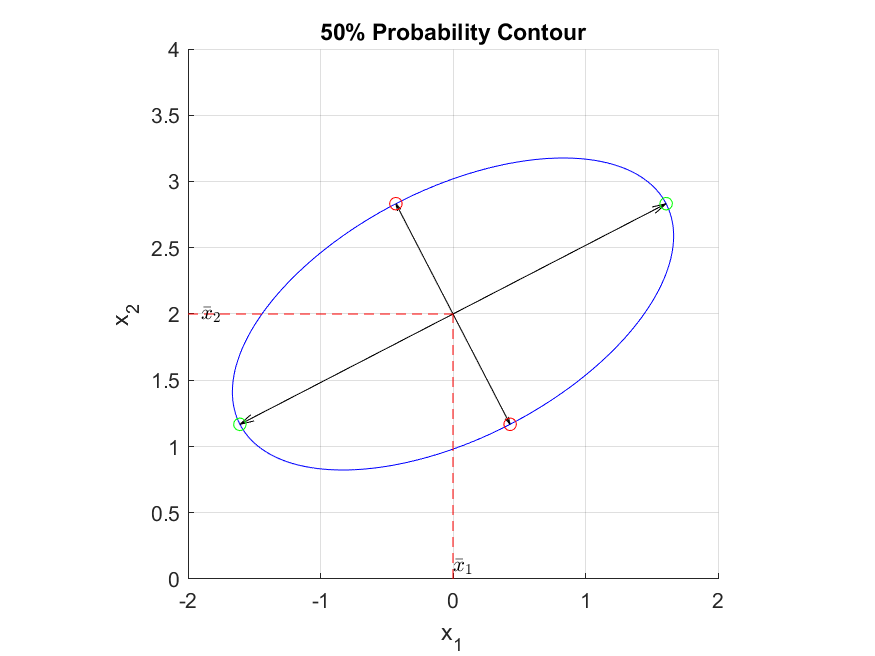
\includegraphics[scale=0.8]{./matlab/chapter-4/sol4.2.png}
\end{figure}
\end{enumerate}
% Let $\textbf{X}$ be $N_3(\bm{\mu},\bm{\Sigma})$ with $\bm{\mu}^{\prime} = [-3,1,4]$ and
\[
    \bm{\Sigma}
    =
    \begin{bNiceArray}{rrr}
        1 & -2 & 0 \\
        -2 & 5 & 0 \\
        0 & 0 & 2
    \end{bNiceArray}
\]
Which of the following random variables are independent? Explain.
\begin{enumerate}[label=(\alph*)]
    \item $X_1$ and $X_2$
    \newline
    \par
    $\text{Cov}(X_1, X_2) = -2 \ne 0$, so no, $X_1$ and $X_2$ are not $\independent$.
    \item $X_2$ and $X_3$
    \newline
    \par
    $\text{Cov}(X_2, X_3) = 0$, so yes, $X_2$ and $X_3$ are $\independent$.
    \item $(X_1, X_2)$ and $X_3$
    \newline
    \par
    If we partition the matrix so that column 3 with rows 1 and 2 make up $\bm{\Sigma}_{12}$,
    \[
        \bm{\Sigma}
        =
        \begin{bNiceArray}{rrr}
            1 & -2 & 0 \\
            -2 & 5 & 0 \\
            0 & 0 & 2 \\
            \CodeAfter \tikz \draw[dotted] (1-|3) -- (4-|3);
            \tikz \draw[dotted] (3-|1) -- (3-|4);
        \end{bNiceArray}
        =
        \begin{bNiceArray}{cc}
            \bm{\Sigma}_{11} & \bm{\Sigma}_{12} \\
            \bm{\Sigma}_{21} & \bm{\Sigma}_{22}
        \end{bNiceArray}
    \]
    \[
        \bm{\Sigma}_{12}
        =
        \begin{bNiceArray}{c}
            0 \\
            0
        \end{bNiceArray}
    \]
    Because $\bm{\Sigma}_{12} = \text{Cov}((X_1, X_2), X_2) = \textbf{0}$, yes, $(X_1, X_2)$ and $X_2$ are $\independent$.
    \item $\frac{X_1 + X_2}{2}$ and $X_3$
    \par
    If we define $Y_1 = \frac{X_1 + X_2}{2}$ and $Y_2 = X_3$ we could then setup $\textbf{A}$ to be
    \[
        \textbf{A}
        =
        \begin{bNiceArray}{rrr}
            \frac{1}{2} & \frac{1}{2} & 0 \\
            0 & 0 & 1 \\
        \end{bNiceArray}
    \]
    \[
        \textbf{A}\textbf{X}
        =
        \begin{bNiceArray}{rrr}
            \frac{1}{2} & \frac{1}{2} & 0 \\
            0 & 0 & 1 \\
        \end{bNiceArray}
        \begin{bNiceArray}{c}
            X_1 \\
            X_2 \\
            X_3
        \end{bNiceArray}
        =
        \begin{bNiceArray}{c}
            \frac{X_1 + X_2}{2} \\
            X_3
        \end{bNiceArray}
        =
        \begin{bNiceArray}{c}
            Y_1 \\
            Y_2
        \end{bNiceArray}
    \]
    \[
        \text{Cov}(\textbf{A}\textbf{X})
        =
        \textbf{A}\text{Cov}(\textbf{X})\textbf{A}^{\prime}
        =
        \begin{bNiceArray}{rrr}
            \frac{1}{2} & \frac{1}{2} & 0 \\
            0 & 0 & 1 \\
        \end{bNiceArray}
        \begin{bNiceArray}{rrr}
            1 & -2 & 0 \\
            -2 & 5 & 0 \\
            0 & 0 & 2
        \end{bNiceArray}
        \begin{bNiceArray}{rr}
            \frac{1}{2} & 0 \\
            \frac{1}{2} & 0 \\
            0 & 1
        \end{bNiceArray}
        =
    \]
    \[
        =
        \begin{bNiceArray}{rrr}
            -\frac{1}{2} & \frac{3}{2} & -2 \\
            0 & 0 & 2 \\
        \end{bNiceArray}
        \begin{bNiceArray}{rr}
            \frac{1}{2} & 0 \\
            \frac{1}{2} & 0 \\
            0 & 1
        \end{bNiceArray}
        =
        \begin{bNiceArray}{cc}
            \frac{1}{2} & 0 \\
            0 & 2
        \end{bNiceArray}
    \]
    Because $\text{Cov}(Y_1,Y_2) = 0$, yes, $\frac{X_1 + X_2}{2}$ and $X_3$ are $\independent$.
    Another way would be to partition the matrix, like in chapter 3
    \[
        \bm{\Sigma}
        =
        \begin{bNiceArray}{rrr}
            1 & -2 & 0 \\
            -2 & 5 & 0 \\
            0 & 0 & 2 \\
            \CodeAfter \tikz \draw[dotted] (1-|3) -- (4-|3);
            \tikz \draw[dotted] (3-|1) -- (3-|4);
        \end{bNiceArray}
        =
        \begin{bNiceArray}{cc}
            \bm{\Sigma}_{11} & \bm{\Sigma}_{12} \\
            \bm{\Sigma}_{21} & \bm{\Sigma}_{22}
        \end{bNiceArray}
    \]
    Then apply a linear combination to $X_1$ and $X_2$, $Y = \textbf{b}^{\prime}\textbf{X}^{\star} = \frac{X_1 + X_2}{2}$, where $\textbf{X}^{\star} = {[X_1, X_2]}^{\prime}$ then
    \[
        \bm{\Sigma}_{11}
        =
        \begin{bNiceArray}{rr}
            1 & -2 \\
            -2 & 5
        \end{bNiceArray},
        \hspace{0.2in}
        \textbf{b}
        =
        \begin{bNiceArray}{c}
            1/2 \\
            1/2
        \end{bNiceArray}
    \]
    \[
        \text{Cov}(Y,X_3)
        =
        \text{Cov}(\textbf{b}^{\prime}\textbf{X}^{\star},X_3)
        =
        \textbf{b}^{\prime}\text{Cov}(\textbf{X}^{\star},X_3)
        =
        \textbf{b}^{\prime}\bm{\Sigma}_{12}
        =
        \begin{bNiceArray}{cc}
            \frac{1}{2} & \frac{1}{2}
        \end{bNiceArray}
        \begin{bNiceArray}{c}
            0 \\
            0
        \end{bNiceArray}
        =
        0
    \]
    Because $\text{Cov}(Y,X_3) = 0$, yes, $Y = \frac{X_1 + X_2}{2}$ and $X_3$ are $\independent$.
    \item $X_2$ and $X_2 - \frac{5}{2}X_1 - X_3$
    \newline
    \par
    If we define $Y_1 = X_2 - \frac{5}{2}X_1 - X_3$ and $Y_2 = X_2$ we could then setup $\textbf{A}$ to be
    \[
        \textbf{A}
        =
        \begin{bNiceArray}{rrr}
            -\frac{5}{2} & 1 & -1 \\
            0 & 1 & 0 \\
        \end{bNiceArray}
    \]
    \[
        \textbf{A}\textbf{X}
        =
        \begin{bNiceArray}{rrr}
            -\frac{5}{2} & 1 & -1 \\
            0 & 1 & 0 \\
        \end{bNiceArray}
        \begin{bNiceArray}{c}
            X_1 \\
            X_2 \\
            X_3
        \end{bNiceArray}
        =
        \begin{bNiceArray}{c}
            X_2 - \frac{5}{2}X_1 - X_3 \\
            X_2
        \end{bNiceArray}
        =
        \begin{bNiceArray}{c}
            Y_1 \\
            Y_2
        \end{bNiceArray}
    \]
    \[
        \text{Cov}(\textbf{A}\textbf{X})
        =
        \textbf{A}\text{Cov}(\textbf{X})\textbf{A}^{\prime}
        =
        \begin{bNiceArray}{rrr}
            -\frac{5}{2} & 1 & -1 \\
            0 & 1 & 0 \\
        \end{bNiceArray}
        \begin{bNiceArray}{rrr}
            1 & -2 & 0 \\
            -2 & 5 & 0 \\
            0 & 0 & 2
        \end{bNiceArray}
        \begin{bNiceArray}{rr}
            -\frac{5}{2} & 0 \\
            1 & 1 \\
            -1 & 0
        \end{bNiceArray}
        =
    \]
    \[
        =
        \begin{bNiceArray}{rrr}
            -\frac{9}{2} & 10 & -2 \\
            -2 & 5 & 0 \\
        \end{bNiceArray}
        \begin{bNiceArray}{rr}
            -\frac{5}{2} & 0 \\
            1 & 1 \\
            -1 & 0
        \end{bNiceArray}
        =
        \begin{bNiceArray}{cc}
            93/4 & 10 \\
            10 & 5
        \end{bNiceArray}
    \]
    Because $\text{Cov}(Y_1,Y_2) = 10$, no, $X_2$ and $X_2 - \frac{5}{2}X_1 - X_3$ are not $\independent$.
\end{enumerate}
% Let $\textbf{X}$ be $N_3(\bm{\mu},\bm{\Sigma})$ with $\bm{\mu} = [2, -3, 1]$ and
\[
    \bm{\Sigma}
    =
    \begin{bNiceArray}{ccc}
        1 & 1 & 1 \\
        1 & 3 & 2 \\
        1 & 2 & 2
    \end{bNiceArray}
\]
\begin{enumerate}[label=(\alph*)]
    \item Find the distribution of $3X_1 - 2X_2 + X_3$.
    \[
        \textbf{b}
        =
        \begin{bNiceArray}{r}
            3 \\
            -2 \\
            1
        \end{bNiceArray},
        \hspace{0.2in}
        \textbf{b}^{\prime}
        \textbf{X}
        =
        \begin{bNiceArray}{rrr}
            3 & -2 & 1
        \end{bNiceArray}
        \begin{bNiceArray}{r}
            X_1 \\
            X_2 \\
            X_3
        \end{bNiceArray}
        =
        3X_1 - 2X_2 + X_3
    \]
    \[
        E[
            \textbf{b}^{\prime}
            \textbf{X}
        ]
        =
        \textbf{b}^{\prime}
        E[
            \textbf{X}
        ]
        =
        \textbf{b}^{\prime}
        \bm{\mu}
        =
        \begin{bNiceArray}{rrr}
            3 & -2 & 1
        \end{bNiceArray}
        \begin{bNiceArray}{r}
            2 \\
            -3 \\
            1
        \end{bNiceArray}
        =
        13
    \]
    \[
        \text{Cov}(
            \textbf{b}^{\prime}
            \textbf{X}
        )
        =
        \textbf{b}^{\prime}
        \text{Cov}
        (
            \textbf{X}
        )
        \textbf{b}
        =
        \textbf{b}^{\prime}
        \bm{\Sigma}
        \textbf{b}
        =
        \begin{bNiceArray}{rrr}
            3 & -2 & 1
        \end{bNiceArray}
        \begin{bNiceArray}{ccc}
            1 & 1 & 1 \\
            1 & 3 & 2 \\
            1 & 2 & 2
        \end{bNiceArray}
        \begin{bNiceArray}{r}
            3 \\
            -2 \\
            1
        \end{bNiceArray}
        =
    \]
    \[
        =
        \begin{bNiceArray}{rrr}
            2 & -1 & 1
        \end{bNiceArray}
        \begin{bNiceArray}{r}
            3 \\
            -2 \\
            1
        \end{bNiceArray}
        =
        9
    \]
    Now we have that
    \[
        \textbf{b}^{\prime}\textbf{X}
        \sim
        N \left(13, 9\right)
    \]
    \item Relabel the variables if necessary, and find a $2 \times 1$ vector $\textbf{a}$ such that $X_2$ and $X_2 - \textbf{a}^{\prime}
    \begin{bNiceArray}{c}
        X_1 \\
        X_2
    \end{bNiceArray}$ are independent.
    \par
    I don't see $X_3$ in $X_2 - \textbf{a}^{\prime}
    \begin{bNiceArray}{c}
        X_1 \\
        X_2
    \end{bNiceArray}$, so if we first partition $\bm{\Sigma}$ and focus on $\bm{\Sigma}_{11}$, that way we're working with only $X_1$ and $X_2$, also defining $\textbf{X}^{\star} = \begin{bNiceArray}{c}
        X_1 \\
        X_2
    \end{bNiceArray}$.
    \[
        \bm{\Sigma}
        =
        \begin{bNiceArray}{ccc}[baseline=2]
            1 & 1 & 1 \\
            1 & 3 & 2 \\
            1 & 2 & 2 \\
            \CodeAfter \tikz \draw[dotted] (3-|1) -- (3-|4);
            \CodeAfter \tikz \draw[dotted] (1-|3) -- (4-|3);
        \end{bNiceArray}
        =
        \begin{bNiceArray}{cc}
            \bm{\Sigma}_{11} & \bm{\Sigma}_{12} \\
            \bm{\Sigma}_{21} & \bm{\Sigma}_{22} \\
            \CodeAfter \tikz \draw[dotted] (2-|1) -- (2-|3);
            \CodeAfter \tikz \draw[dotted] (1-|2) -- (3-|2);
        \end{bNiceArray}
    \]
    \[
        X_2 - \textbf{a}^{\prime}
        \begin{bNiceArray}{c}
            X_1 \\
            X_2
        \end{bNiceArray}
        =
        X_2 
        - 
        a_1 X_1
        -
        a_2 X_2
        =
        -a_1 X_1
        +
        (1 - a_2)
        X_2
        =
        \begin{bNiceArray}{rr}
            -a_1 & (1 - a_2)
        \end{bNiceArray}
        \begin{bNiceArray}{c}
            X_1 \\
            X_2
        \end{bNiceArray}
    \]
    We're interested in the covariance of $X_2$ with this, so we can setup $\textbf{A}$ to be
    \[
        A
        =
        \begin{bNiceArray}{cc}
            0 & 1 \\
            -a_1 & (1 - a_2)
        \end{bNiceArray}
    \]
    \[
        \text{Cov}(
            \textbf{A}
            \textbf{X}^{\star}
        )
        =
        \textbf{A}
        \text{Cov}
        (
            \textbf{X}^{\star}
        )
        \textbf{A}^{\prime}
        =
        \textbf{A}
        \bm{\Sigma}_{11}
        \textbf{A}^{\prime}
        =
    \]
    \[
        =
        \begin{bNiceArray}{cc}
            0 & 1 \\
            -a_1 & (1 - a_2)
        \end{bNiceArray}
        \begin{bNiceArray}{cc}
            1 & 1 \\
            1 & 3
        \end{bNiceArray}
        \begin{bNiceArray}{cc}
            0 & -a_1 \\
            1 & (1 - a_2)
        \end{bNiceArray}
        =
    \]
    \[
        =
        \begin{bNiceArray}{cc}
            1 & 3 \\
            -a_1 & (3 - a_1 - 3 a_2)
        \end{bNiceArray}
        \begin{bNiceArray}{cc}
            0 & -a_1 \\
            1 & (1 - a_2)
        \end{bNiceArray}
        =
    \]
    \[
        =
        \begin{bNiceArray}{cc}
            1 & (3 - a_1 - 3 a_2) \\
            (3 - a_1 - 3 a_2) & (a_1^2 + (1-a_2)(3 - a_1 - 3 a_2))
        \end{bNiceArray}
    \]
    We want to know when $X_2$ and $X_2 - \textbf{a}^{\prime}
    \begin{bNiceArray}{c}
        X_1 \\
        X_2
    \end{bNiceArray}$ are independent. This is when the off-diagonal elements of this covariance matrix are zero, that is, when
    \[
        3 - a_1 - 3 a_2 = 0 \Rightarrow a_1 + 3 a_2 = 3
    \]
    If we pick $a_1 = 1$, then $a_2 = \frac{2}{3}$ and $
        \textbf{a}
        =
        \begin{bNiceArray}{c}
            a_1 \\
            a_2
        \end{bNiceArray}
        =
        \begin{bNiceArray}{c}
            1 \\
            \frac{2}{3}
        \end{bNiceArray}
    $.
    Now to check that this is correct.
    \[
        A
        =
        \begin{bNiceArray}{cc}
            0 & 1 \\
            -1 & \left(1 - \frac{2}{3}\right)
        \end{bNiceArray}
        =
        \begin{bNiceArray}{cc}
            0 & 1 \\
            -1 & \frac{1}{3}
        \end{bNiceArray}
    \]
    \[
        \text{Cov}(
            \textbf{A}
            \textbf{X}^{\star}
        )
        =
        \textbf{A}
        \text{Cov}
        (
            \textbf{X}^{\star}
        )
        \textbf{A}^{\prime}
        =
        \textbf{A}
        \bm{\Sigma}_{11}
        \textbf{A}^{\prime}
        =
    \]
    \[
        =
        \begin{bNiceArray}{cc}
            0 & 1 \\
            -1 & \frac{1}{3}
        \end{bNiceArray}
        \begin{bNiceArray}{cc}
            1 & 1 \\
            1 & 3
        \end{bNiceArray}
        \begin{bNiceArray}{cc}
            0 & -1 \\
            1 & \frac{1}{3}
        \end{bNiceArray}
        =
        \begin{bNiceArray}{cc}
            1 & 3 \\
            -\frac{2}{3} & 0
        \end{bNiceArray}
        \begin{bNiceArray}{cc}
            0 & -1 \\
            1 & \frac{1}{3}
        \end{bNiceArray}
        =
        \begin{bNiceArray}{cc}
            3 & 0 \\
            0 & \frac{2}{3}
        \end{bNiceArray}
    \]
    The off-diagonal values are zero, so $\text{Cov}(X_2, X_2 - \textbf{a}^{\prime}\begin{bNiceArray}{c}
        X_1 \\
        X_2
    \end{bNiceArray}) = 0$ and are $\independent$.
\end{enumerate}
% Specify the following.
\begin{enumerate}[label= (\alph*)]
    \item The conditional distribution of $X_1$, given that $X_2 = x_2$ for the joint distribution in Exercise 4.2.
    \[
        \bm{\mu}
        =
        \begin{bNiceArray}{c}
            \mu_1 \\
            \mu_2
        \end{bNiceArray}
        =
        \begin{bNiceArray}{c}
            0 \\
            2
        \end{bNiceArray}
    \]
    \[
        \bm{\Sigma}
        =
        \begin{bNiceArray}{cc}
            \sigma_{11} & \sigma_{12} \\
            \sigma_{21} & \sigma_{22}
        \end{bNiceArray}
        =
        \begin{bNiceArray}{cc}
            \sigma_{11} & \rho_{12}\sqrt{\sigma_{11}}\sqrt{\sigma_{22}} \\
            \rho_{12}\sqrt{\sigma_{11}}\sqrt{\sigma_{22}} & \sigma_{22}
        \end{bNiceArray}
        =
        \begin{bNiceArray}{cc}
            2 & \sqrt{2}/2 \\
            \sqrt{2}/2 & 1
        \end{bNiceArray}
    \]
    Using \textbf{Result 4.6} on page 160, the conditional distribution is normally distributed with
    \[
        \text{Mean}
        =
        \mu_1
        +
        \sigma_{12}\sigma_{22}^{-1}(x_2 - \mu_2)
        =
        0
        +
        \left(\frac{\sqrt{2}}{2}\right)\left(\frac{1}{1}\right)(x_2 - 2)
        =
        \frac{\sqrt{2}}{2}(x_2 - 2)
    \]
    \[
        \text{Covariance}
        =
        \sigma_{11}
        -
        \sigma_{12}\sigma_{22}^{-1}\sigma_{21}
        =
        2
        -
        \left(\frac{\sqrt{2}}{2}\right)
        \left(\frac{1}{1}\right)
        \left(\frac{\sqrt{2}}{2}\right)
        =
        2
        -
        \frac{2}{4}
        =
        \frac{3}{2}
    \]
    \[
        X_1 \bigg{|}
        X_2 = x_2
        \sim
        N \left(\frac{\sqrt{2}}{2}(x_2 - 2),\frac{3}{2}\right)
    \]
    \item The conditional distribution of $X_2$, given that $X_1 = x_1$ and $X_3 = x_3$ for the joint distribution in Exercise 4.3.
    \[
        \bm{\mu}
        =
        \begin{bNiceArray}{c}
            \mu_1 \\
            \mu_2 \\
            \mu_3
        \end{bNiceArray}
        =
        \begin{bNiceArray}{r}
            -3 \\
            1 \\
            4
        \end{bNiceArray}
        ,\hspace{0.2in}
        \bm{\Sigma}
        =
        \begin{bNiceArray}{rrr}
            1 & -2 & 0 \\
            -2 & 5 & 0 \\
            0 & 0 & 2
        \end{bNiceArray}
    \]
    This time we need to rearrange the rows and columns so that $X_2$ is the first row and the first column. Then, from \textbf{Result 4.4} on page 158, the subsets of a normal are also normal, and again, using \textbf{Result 4.6} to find the mean and variance of the normal for the conditional distribution.
    \[
        \bm{\mu}
        =
        \begin{bNiceArray}{c}
            \mu_2 \\
            \mu_1 \\
            \mu_3 \\
            \CodeAfter \tikz \draw[dotted] (2-|1) -- (2|-2);
        \end{bNiceArray}
        =
        \begin{bNiceArray}{r}
            1 \\
            -3 \\
            4 \\
            \CodeAfter \tikz \draw[dotted] (2-|1) -- (2|-2);
        \end{bNiceArray}
        =
        \begin{bNiceArray}{c}
            \bm{\mu}_1 \\
            \bm{\mu}_2 \\
            \CodeAfter \tikz \draw[dotted] (2-|1) -- (2|-2);
        \end{bNiceArray}
    \]
    \[
        \bm{\Sigma}
        =
        \begin{bNiceArray}{rrr}
            1 & -2 & 0 \\
            -2 & 5 & 0 \\
            0 & 0 & 2
        \end{bNiceArray}
        \xrightarrow{
            \begin{subarray}{c}
                \text{Swap row 1 and row 2} \\
                \text{Swap column 1 and column 2}
            \end{subarray}
        }
        \begin{bNiceArray}{rrr}
            5 & -2 & 0 \\
            -2 & 1 & 0 \\
            0 & 0 & 2 \\
            \CodeAfter \tikz \draw[dotted] (2-|1) -- (2-|4);
            \tikz \draw[dotted] (1-|2) -- (4-|2);
        \end{bNiceArray}
        =
        \begin{bNiceArray}{rr}
            \bm{\Sigma}_{11} & \bm{\Sigma}_{12} \\
            \bm{\Sigma}_{21} & \bm{\Sigma}_{22} \\
            \CodeAfter \tikz \draw[dotted] (2-|1) -- (2-|3);
            \tikz \draw[dotted] (1-|2) -- (3-|2);
        \end{bNiceArray}
    \]
    The conditional distribution is normally distributed with
    \[
        \text{Mean}
        =
        \bm{\mu}_1
        + 
        \bm{\Sigma}_{12}
        \bm{\Sigma}_{22}^{-1}
        (\textbf{x}_2 - \bm{\mu}_2)
        =
        1
        +
        \begin{bNiceArray}{rr}
            -2 & 0
        \end{bNiceArray}
        \begin{bNiceArray}{rr}
            1 & 0 \\
            0 & \frac{1}{2}
        \end{bNiceArray}
        \left(
            \begin{bNiceArray}{c}
                x_1 \\
                x_3
            \end{bNiceArray}
            -
            \begin{bNiceArray}{c}
                1 \\
                4
            \end{bNiceArray}
        \right)
        =
    \]
    \[
        =
        1
        +
        \begin{bNiceArray}{rr}
            -2 & 0
        \end{bNiceArray}
        \begin{bNiceArray}{c}
            \left(x_1 - 1\right) \\
            \left(x_3 - 4\right)
        \end{bNiceArray}
        =
        1
        -
        2
        \left(x_1 - 1\right)
        =
        3 - 2 x_1
    \]
    \[
        \text{Covariance}
        =
        \bm{\Sigma}_{11}
        -
        \bm{\Sigma}_{12}
        \bm{\Sigma}_{22}^{-1}
        \bm{\Sigma}_{21}
        =
        5
        -
        \begin{bNiceArray}{rr}
            -2 & 0
        \end{bNiceArray}
        \begin{bNiceArray}{rr}
            1 & 0 \\
            0 & \frac{1}{2}
        \end{bNiceArray}
        \begin{bNiceArray}{r}
            -2 \\
            0
        \end{bNiceArray}
        =
    \]
    \[
        =
        5-
        \begin{bNiceArray}{rr}
            -2 & 0
        \end{bNiceArray}
        \begin{bNiceArray}{r}
            -2 \\
            0
        \end{bNiceArray}
        =
        5
        -
        4
        =
        1
    \]
    \[
        X_2 \bigg{|}
        X_1 = x_1, X_3 = x_3
        \sim
        N\bigg{(}( 3 -2 x_1 ),1\bigg{)}
    \]
    \item The conditional distribution of $X_3$, given that $X_1 = x_1$ and $X_2 = x_2$ for the joint distribution in Exercise 4.4.
    \[
        \bm{\mu}
        =
        \begin{bNiceArray}{c}
            \mu_1 \\
            \mu_2 \\
            \mu_3
        \end{bNiceArray}
        =
        \begin{bNiceArray}{r}
            2 \\
            -3 \\
            1
        \end{bNiceArray}
        ,\hspace{0.2in}
        \bm{\Sigma}
        =
        \begin{bNiceArray}{rrr}
            1 & 1 & 1 \\
            1 & 3 & 2 \\
            1 & 2 & 2
        \end{bNiceArray}
    \]
    This time, again, we need to rearrange the rows and columns of $\bm{\mu}$ and $\bm{\Sigma}$. For this conditional distribution we need to partition so that $X_3$ is the first row and the first column. From \textbf{Result 4.4}, the subsets of the normal are also normal, and using \textbf{Result 4.6} to get the conditional distribution.
    \[
        \bm{\mu}
        =
        \begin{bNiceArray}{c}
            \mu_3 \\
            \mu_1 \\
            \mu_2 \\
            \CodeAfter \tikz \draw[dotted] (2-|1) -- (2|-2);
        \end{bNiceArray}
        =
        \begin{bNiceArray}{r}
            1 \\
            2 \\
            -3 \\
            \CodeAfter \tikz \draw[dotted] (2-|1) -- (2|-2);
        \end{bNiceArray}
        =
        \begin{bNiceArray}{c}
            \bm{\mu}_1 \\
            \bm{\mu}_2 \\
            \CodeAfter \tikz \draw[dotted] (2-|1) -- (2|-2);
        \end{bNiceArray}
    \]
    \[
        \bm{\Sigma}
        =
        \begin{bNiceArray}{rrr}
            \sigma_{11} & \sigma_{12} & \sigma_{13} \\
            \sigma_{21} & \sigma_{22} & \sigma_{23} \\
            \sigma_{31} & \sigma_{32} & \sigma_{33} \\
        \end{bNiceArray}
        \xrightarrow{
            \begin{subarray}{c}
                \text{Move row 3 and row 1} \\
                \text{Move column 3 to column 1}
            \end{subarray}
        }
        \begin{bNiceArray}{rrr}
            \sigma_{33} & \sigma_{31} & \sigma_{32} \\
            \sigma_{13} & \sigma_{11} & \sigma_{12} \\
            \sigma_{23} & \sigma_{21} & \sigma_{22} \\
        \end{bNiceArray}
        =
    \]
    \[
        =
        \begin{bNiceArray}{rrr}
            2 & 1 & 2 \\
            1 & 1 & 1 \\
            2 & 1 & 3 \\
            \CodeAfter \tikz \draw[dotted] (2-|1) -- (2-|4);
            \tikz \draw[dotted] (1-|2) -- (4-|2);
        \end{bNiceArray}
        =
        \begin{bNiceArray}{rr}
            \bm{\Sigma}_{11} & \bm{\Sigma}_{12} \\
            \bm{\Sigma}_{21} & \bm{\Sigma}_{22} \\
            \CodeAfter \tikz \draw[dotted] (2-|1) -- (2-|3);
            \tikz \draw[dotted] (1-|2) -- (3-|2);
        \end{bNiceArray}
    \]
    The conditional distribution is normally distributed with
    \[
        \text{Mean}
        =
        \bm{\mu}_1
        + 
        \bm{\Sigma}_{12}
        \bm{\Sigma}_{22}^{-1}
        (\textbf{x}_2 - \bm{\mu}_2)
        =
        1
        +
        \begin{bNiceArray}{rr}
            1 & 2
        \end{bNiceArray}
        \begin{bNiceArray}{rr}
            3/2 & -1/2 \\
            -1/2 & 1/2
        \end{bNiceArray}
        \left(
            \begin{bNiceArray}{c}
                x_1 \\
                x_2
            \end{bNiceArray}
            -
            \begin{bNiceArray}{r}
                2 \\
                -3
            \end{bNiceArray}
        \right)
        =
    \]
    \[
        =
        1
        +
        \begin{bNiceArray}{rr}
            1/2 & 1/2
        \end{bNiceArray}
        \begin{bNiceArray}{c}
            \left(x_1 - 2\right) \\
            \left(x_2 + 3\right)
        \end{bNiceArray}
        =
        \frac{1}{2} x_1
        +
        \frac{1}{2} x_2
        +
        \frac{3}{2}
    \]
    \[
        \text{Covariance}
        =
        \bm{\Sigma}_{11}
        -
        \bm{\Sigma}_{12}
        \bm{\Sigma}_{22}^{-1}
        \bm{\Sigma}_{21}
        =
        2
        -
        \begin{bNiceArray}{rr}
            1 & 2
        \end{bNiceArray}
        \begin{bNiceArray}{rr}
            3/2 & -1/2 \\
            -1/2 & 1/2
        \end{bNiceArray}
        \begin{bNiceArray}{r}
            1 \\
            2
        \end{bNiceArray}
        =
    \]
    \[
        =
        2
        -
        \begin{bNiceArray}{rr}
            1/2 & 1/2
        \end{bNiceArray}
        \begin{bNiceArray}{r}
            1 \\
            2
        \end{bNiceArray}
        =
        2
        -
        \frac{3}{2}
        =
        \frac{1}{2}
    \]
    \[
        X_3 \bigg{|}
        X_1 = x_1, X_2 = x_2
        \sim
        N \left( \frac{1}{2}(x_1 + x_2 + 3), \frac{1}{2} \right)
    \]
\end{enumerate}
% Let $\textbf{X}$ be distributed as $N_{3} (\bm{\mu}, \bm{\Sigma})$, where $\bm{\mu}^{\prime} = [1, -1, 2]$ and
\[
    \bm{\Sigma}
    =
    \begin{bNiceArray}{rrr}
        4 & 0 & -1 \\
        0 & 5 & 0 \\
        -1 & 0 & 2
    \end{bNiceArray}
\]
Which of the following random variables are independent? Explain.
\begin{enumerate}[label= (\alph*)]
    \item $X_1$ and $X_2$
    \par
    Picking out the value of $\text{Cov}(X_1, X_2) = \sigma_{12} = \sigma_{21}$ from $\bm{\Sigma}$, we can see that $\text{Cov}(X_1, X_2) = 0$, so by part \textbf{(a)} of \textbf{Result 4.5} on page 159 $X_1$ and $X_2$ are $\independent$.
    \item $X_1$ and $X_3$
    \par
    Picking out the value of $\text{Cov}(X_1, X_3) = \sigma_{13} = \sigma_{31}$ from $\bm{\Sigma}$, we can see that $\text{Cov}(X_1, X_3) = -1$, so by part \textbf{(a)} of \textbf{Result 4.5} on page 159 $X_1$ and $X_3$ are not $\independent$.
    \item $X_2$ and $X_3$
    \par
    Picking out the value of $\text{Cov}(X_2, X_3) = \sigma_{23} = \sigma_{32}$ from $\bm{\Sigma}$, we can see that $\text{Cov}(X_2, X_3) = 0$, so by part \textbf{(a)} of \textbf{Result 4.5} on page 159 $X_2$ and $X_3$ are $\independent$.
    \item $(X_1, X_3)$ and $X_2$
    \par
    This time partition $\bm{\mu}$ and $\bm{\Sigma}$ so that $X_2$ is the last row of $\bm{\mu}$ and the last row/column of $\bm{\Sigma}$
    \[
        \bm{\mu}
        =
        \begin{bNiceArray}{r}
            \mu_1 \\
            \mu_2 \\
            \mu_3
        \end{bNiceArray}
        =
        \begin{bNiceArray}{r}
            \mu_1 \\
            \mu_3 \\
            \mu_2 \\
            \CodeAfter \tikz \draw[dotted] (3-|1) -- (3-|2);
        \end{bNiceArray}
        =
        \begin{bNiceArray}{r}
            1 \\
            2 \\
            -1 \\
            \CodeAfter \tikz \draw[dotted] (3-|1) -- (3-|2);
        \end{bNiceArray}
        =
        \begin{bNiceArray}{r}
            \bm{\mu}_1 \\
            \bm{\mu}_2 \\
            \CodeAfter \tikz \draw[dotted] (2-|1) -- (2-|2);
        \end{bNiceArray}
    \]
    \[
        \bm{\Sigma}
        =
        \begin{bNiceArray}{ccc}
            \sigma_{11} & \sigma_{12} & \sigma_{13} \\
            \sigma_{21} & \sigma_{22} & \sigma_{23} \\
            \sigma_{31} & \sigma_{32} & \sigma_{33}
        \end{bNiceArray}
        \xrightarrow{
            \begin{subarray}{c}
                \text{Swap column 2 and column 3} \\
                \text{Swap row 2 and row 3}
            \end{subarray}
        }
        \begin{bNiceArray}{ccc}
            \sigma_{11} & \sigma_{13} & \sigma_{12} \\
            \sigma_{31} & \sigma_{33} & \sigma_{32} \\
            \sigma_{21} & \sigma_{23} & \sigma_{22} \\
            \CodeAfter \tikz \draw[dotted] (3-|1) -- (3-|4);
            \tikz \draw[dotted] (1-|3) -- (4-|3);
        \end{bNiceArray}
        =
    \]
    \[
        =
        \begin{bNiceArray}{rrr}
            4 & -1 & 0 \\
            -1 & 2 & 0 \\
            0 & 0 & 5 \\
            \CodeAfter \tikz \draw[dotted] (3-|1) -- (3-|4);
            \tikz \draw[dotted] (1-|3) -- (4-|3);
        \end{bNiceArray}
        =
        \begin{bNiceArray}{cc}
            \bm{\Sigma_{11}} & \bm{\Sigma_{12}} \\
            \bm{\Sigma_{21}} & \bm{\Sigma_{22}} \\
            \CodeAfter \tikz \draw[dotted] (2-|1) -- (2-|3);
            \tikz \draw[dotted] (1-|2) -- (3-|2);
        \end{bNiceArray}
    \]
    Here, $\textbf{X}_1 = \begin{bNiceArray}{c} X_1 \\ X_3 \end{bNiceArray}$ and $\textbf{X}_2 = \begin{bNiceArray}{c} X_2 \end{bNiceArray}$. Picking out the value of $\text{Cov}(\textbf{X}_1, \textbf{X}_2) = \bm{\Sigma}_{12} = \begin{bNiceArray}{c} 0 \\ 0 \end{bNiceArray} = \textbf{0}$ from the partitioned $\bm{\Sigma}$, we can see that $\bm{\Sigma}_{12} = \textbf{0}$, so by part \textbf{(b)} of \textbf{Result 4.5} on page 159 $(X_1, X_3)$ and $X_2$ are $\independent$.

    \item $X_1$ and $X_1 + 3X_2 - 2X_3$
    \par
    For this, we have $q = 2$ linear combinations, so
    \[
        \textbf{A}
        =
        \begin{bNiceArray}{c}
            \textbf{a}_{1}^{\prime} \\
            \textbf{a}_{2}^{\prime}
        \end{bNiceArray}
        =
        \begin{bNiceArray}{rrr}
            1 & 0 & 0 \\
            1 & 3 & -2
        \end{bNiceArray}
    \]
    From \textbf{Result 4.3} on page 157, this would be distributed as $N_{q} (,(\textbf{A}\bm{\mu}, \textbf{A}\bm{\Sigma}\textbf{A}^{\prime})$. Computing $\textbf{A}\bm{\Sigma}\textbf{A}^{\prime}$ we have
    \[
        \textbf{A}\bm{\Sigma}\textbf{A}^{\prime}
        =
        \begin{bNiceArray}{rrr}
            1 & 0 & 0 \\
            1 & 3 & -2
        \end{bNiceArray}
        \begin{bNiceArray}{rrr}
            4 & 0 & -1 \\
            0 & 5 & 0 \\
            -1 & 0 & 2
        \end{bNiceArray}
        \begin{bNiceArray}{rr}
            1 & 1 \\
            0 & 3 \\
            0 & -2
        \end{bNiceArray}
        =
        \begin{bNiceArray}{rrr}
            4 & 0 & -1 \\
            6 & 15 & -5
        \end{bNiceArray}
        \begin{bNiceArray}{rr}
            1 & 1 \\
            0 & 3 \\
            0 & -2
        \end{bNiceArray}
        =
    \]
    \[
        =
        \begin{bNiceArray}{rr}
            4 & 6 \\
            6 & 61
        \end{bNiceArray}
    \]
    This is the variance-covariance matrix of $X_1$ and $X_1 + 3X_2 - 2X_3$. Picking out the off-diagonal term, $\text{Cov}(X_1, X_1 + 3X_2 - 2X_3) = 6$. This value is not zero, so by \textbf{Result 4.5} part \textbf{(a)}, $X_1$ and $X_1 + 3X_2 - 2X_3$ are not $\independent$.
\end{enumerate}
% Refer to Exercise 4.6 and specify each of the following.
\begin{enumerate}[label= (\alph*)]
    \item The conditional distribution of $X_1$, given that $X_3 = x_3$.
    \par
    We only care about $X_1$ and $X_3$, so to remove $X_2$ we could first apply the linear combinations
    \[
        \textbf{A}
        =
        \begin{bNiceArray}{ccc}
            1 & 0 & 0 \\
            0 & 0 & 1
        \end{bNiceArray}
    \]
    so by \textbf{Result 4.3}, this would be distributed as $N_{2}(\textbf{A}\bm{\mu}, \textbf{A}\bm{\Sigma}\textbf{A}^{\prime})$, where
    \[
        \textbf{A}\bm{\mu}
        =
        \begin{bNiceArray}{c}
            1 \\
            2
        \end{bNiceArray}
        =
        \begin{bNiceArray}{c}
            \mu_1 \\
            \mu_3
        \end{bNiceArray}
        \hspace{0.2in}\text{and}\hspace{0.2in}
        \textbf{A}\bm{\Sigma}\textbf{A}^{\prime}
        =
        \begin{bNiceArray}{rr}
            4 & -1 \\
            -1 & 2
        \end{bNiceArray}
        =
        \begin{bNiceArray}{cc}
            \sigma_{11} & \sigma_{13} \\
            \sigma_{31} & \sigma_{33}
        \end{bNiceArray}
    \]
    From here we can use \textbf{Result 4.6} to get the conditional distribution
    \[
        \text{Mean}
        =
        \mu_1
        +
        \sigma_{13}
        \sigma_{33}^{-1}
        (x_3 - \mu_3)
        =
        1
        +
        (-1)
        (1/2)
        (x_3 - 2)
        =
        2
        -
        \frac{1}{2}
        x_3
    \]
    \[
        \text{Covariance}
        =
        \sigma_{11}
        +
        \sigma_{13}
        \sigma_{33}^{-1}
        \sigma_{31}
        =
        4
        -
        {(-1)}^2
        (1/2)
        -
        4
        -
        1/2
        =
        \frac{7}{2}
    \]
    and putting it together we have
    \[
        X_1 \bigg{|} X_3 = x_3
        \sim
        N \left(
            2 - \frac{1}{2} x_3,
            \frac{7}{2}
        \right)
    \]
    \item The conditional distribution of $X_1$, given that $X_2 = x_2$ and $X_3 = x_3$.
    \par
    This time partition things so that one group contains $X_1$ and another group contains $X_2$ and $X_3$.
    \[
        \bm{\mu}
        =
        \begin{bNiceArray}{r}
            1 \\
            -1 \\
            2
        \end{bNiceArray}
        =
        \begin{bNiceArray}{r}
            1 \\
            -1 \\
            2 \\
            \CodeAfter \tikz \draw[dotted] (2-|1) -- (2|-2);
        \end{bNiceArray}
        =
        \begin{bNiceArray}{c}
            \bm{\mu}_{1} \\
            \bm{\mu}_{2} \\
            \CodeAfter \tikz \draw[dotted] (2-|1) -- (2|-2);
        \end{bNiceArray}
    \]
    \[
        \bm{\mu}
        =
        \begin{bNiceArray}{rrr}
            4 & 0 & -1 \\
            0 & 5 & 0 \\
            -1 & 0 & 2
        \end{bNiceArray}
        =
        \begin{bNiceArray}{rrr}
            4 & 0 & -1 \\
            0 & 5 & 0 \\
            -1 & 0 & 2 \\
            \CodeAfter \tikz \draw[dotted] (2|-1) -- (2|-4);
            \tikz \draw[dotted] (1|-2) -- (4|-2);
        \end{bNiceArray}
        =
        \begin{bNiceArray}{rrr}
            \bm{\Sigma}_{11} & \bm{\Sigma}_{12} \\
            \bm{\Sigma}_{21} & \bm{\Sigma}_{22} \\
            \CodeAfter \tikz \draw[dotted] (2|-1) -- (2|-3);
            \tikz \draw[dotted] (1|-2) -- (3|-2);
        \end{bNiceArray}
    \]
    Again, apply \textbf{Result 4.6},
    \[
        \text{Mean}
        =
        \bm{\mu}_1
        +
        \bm{\Sigma}_{12}
        \bm{\Sigma}_{22}^{-1}
        \left(\textbf{x}_2 - \bm{\mu}_2\right)
        =
        1
        +
        \begin{bNiceArray}{rr}
            0 & -1
        \end{bNiceArray}
        \begin{bNiceArray}{rr}
            2/10 & 0 \\
            0 & 5/10
        \end{bNiceArray}
        \left(
            \begin{bNiceArray}{c}
                x_2 \\
                x_3
            \end{bNiceArray}
            -
            \begin{bNiceArray}{r}
                -1 \\
                2
            \end{bNiceArray}
        \right)
        =
    \]
    \[
        =
        1
        +
        \begin{bNiceArray}{rr}
            0 & -1/2
        \end{bNiceArray}
        \begin{bNiceArray}{c}
            x_2 + 1 \\
            x_3 - 2
        \end{bNiceArray}
        =
        1
        -
        \frac{1}{2}
        \left(
            x_3 - 2
        \right)
        =
        2
        -
        \frac{1}{2}
        x_3
    \]
    \[
        \text{Covariance}
        =
        \bm{\Sigma}_{11}
        -
        \bm{\Sigma}_{12}
        \bm{\Sigma}_{11}^{-1}
        \bm{\Sigma}_{21}
        =
        4
        -
        \begin{bNiceArray}{rr}
            0 & -1
        \end{bNiceArray}
        \begin{bNiceArray}{rr}
            2/10 & 0 \\
            0 & 5/10
        \end{bNiceArray}
        \begin{bNiceArray}{r}
            0 \\
            -1
        \end{bNiceArray}
        =
    \]
    \[
        =
        4
        -
        \begin{bNiceArray}{rr}
            0 & -1/2
        \end{bNiceArray}
        \begin{bNiceArray}{r}
            0 \\
            -1
        \end{bNiceArray}
        =
        4
        -
        \frac{1}{2}
        =
        \frac{7}{2}
    \]
    Putting this together we have
    \[
        X_1 \bigg{|} X_2, X_3
        \sim
        \left(
            2
            -
            \frac{1}{2}
            x_3,
            \frac{7}{2}
        \right)
    \]
\end{enumerate}
% (Example of a nonnormal bivariate distribution with normal marginals.) Let $X_1$ be $N(0,1)$ and let
\[
  X_2
  =
  \begin{cases*}
    -X_1 & if $-1 \leq X_1 \leq 1$ \\
    \phantom{-}X_1 & otherwise
  \end{cases*}
\]
Show each of the following.
\begin{enumerate}[label= (\alph*)]
    \item $X_2$ also has an $N(0,1)$ distribution.
    \par
    The hint is basically the answer. Using symmetry we can start with
    \[
      P (-1 < X_1 \leq x)
      =
      P(-x \leq X_1 < 1)
    \]
    Using the definition of the CDF for $X_2$
    \begin{align*}
      F_{X_2}(x_2)
      =
      \\
      =
      P (X_2 \leq x_2)
      =
      \\
      =
      P (X_2 \leq -1)
      +
      P (-1 < X_2 \leq x_2)
      = 
      \\
      =
      P (X_1 \leq -1)
      +
      P (-1 < -X_1 \leq x_2)
      = \tag*{Using the definition of $X_2$.}
      \\
      =
      P (X_1 \leq -1)
      +
      P (-x_2 \leq X_1 < 1)
      =
      \\
      =
      P (X_1 \leq -1)
      +
      P (-1 < -X_1 \leq x_2)
      = \tag*{Using symmetry argument.}
      \\
      P (X_1 \leq x_2) \tag*{CDF definition for $X_1$.}
      =
      \\
      F_{X_1}(x_2)
    \end{align*}
    The CDF for $X_1$ and $X_2$ are the same, so since $X_1 \sim N(0,1)$, then $X_2$ is also distributed as $N(0,1)$.
    
    \item $X_1$ and $X_2$ do \textit{not} have a bivariate normal distribution.
    \[
      \textbf{a}
      =
      \begin{bNiceArray}{r}
        1 \\
        -1
      \end{bNiceArray}
      ,\hspace{0.2in}
      \textbf{X}
      =
      \begin{bNiceArray}{r}
        X_1 \\
        X_2
      \end{bNiceArray}
      ,\hspace{0.2in}
      Y
      =
      \textbf{a}^{\prime}
      \textbf{X}
      =
      X_1 - X_2
    \]
    \[
        \textbf{a}^{\prime}
        \textbf{X}
      =
        X_1 - X_2
      =
      \begin{cases*}
        X_1 - (-X_1) & if $-1 \leq X_1 \leq 1$ \\
        X_1 - X_1 & otherwise
      \end{cases*}
      =
    \]
    \[
      =
      \begin{cases*}
        2X_1 & if $-1 \leq X_1 \leq 1$ \\
        0 & otherwise
      \end{cases*}
    \]
    If $X_1$ is in the interval $-1 \leq X_1 \leq 1$ then it's distribution as $ Y = (X_1 - X_2) \sim N(0,4)$, since $E[\textbf{a}^{\prime}\textbf{X}] = E[2X_1] = 2E[X_1]=2\mu_1=2*0 = 0$ and $V[\textbf{a}^{\prime}\textbf{X}] = V[2X_1] = 4V[X_1] = 4\sigma_1^2 = 4*1 = 4$.
    But if $X_1$ is not in the interval $-1 \leq X_1 \leq 1$, then $X_1 - X_2 = 0$. This happens with point probability

    \[
      P(
        \textbf{a}^{\prime}
        \textbf{X}
      )
      =
      P(X_1 - X_2)
      =
      P(0)
      =
      P(X_1 < -1 \text{ and } X_1 > 1)
      =
    \]
    \[
      =
      P(X_1 < -1) + P(X_1 > 1)
      =
      2P(X_1 > 1)
      =
      P(|X_1| > 1)
      =
      0.3173105
    \]
    So since $P(0) \ne 0$, $X_1$ and $X_2$ don't have a bivariate normal. Basically, a Normal distribution is either entirely continuous or entirely discrete, so here we have a discrete point mass at 0 that doesn't have a probability of zero and a continuous $N(0,4)$ distribution from -2 to 2, so this is not consistent with a normal distribution.
    \par The R code for this probability calculation is \texttt{2*pnorm(1, lower.tail=FALSE)}. Could have also done the probability calculation as
    \[
      P(|X_1| > 1)
      =
      1 - P(|X_1| \leq 1)
      =
      1 - P(-1 \leq X_1 \leq 1)
      =
    \]
    \[
      =
      1 - \left( \Phi (1) - \Phi (-1) \right)
      =
      1 - 0.6826895
      =0.3173105
    \]
    Where $\Phi$ is the CDF of a standard normal distribution. The R code is \texttt{1 - (pnorm(1)- pnorm(-1))}.
    \newline
    \textit{Hint:}
    \begin{enumerate}[label= (\alph*)]
        \item Since $X_1$ is $N(0,1)$, $P[-1 < X_1 \leq x] = P[-x \leq X_1 < 1]$ for any $x$. When $-1 < x_2 < 1$, $P[X_2 \leq x_2] = P[X_2 \leq -1] + P[-1 < X_2 \leq x_2] = P[X_1 \leq -1] + P[-1 < -X_1 \leq x_2] = P[X_1 \leq -1] + P[-x_2 \leq X_1 < 1]$. But $P[-x_2 \leq X_1 < 1] = P[-1 < X_1 \leq x_2]$ from the symmetry argument in the first line of this hint. Thus $P[X_2 \leq x_2] = P[X_1 \leq -1] + P[-1 < X_1 \leq x_2] = P[X_1 \leq x_2]$, which is a standard normal probability.
        \item Consider the linear combination $X_1 - X_2$, which equals zero with probability $P[|X_1| > 1] = 0.3174$.
    \end{enumerate}
\end{enumerate}
 % 4.8 Important!
% Refer to Exercise 4.8, but modify the construction by replacing the break point 1 by $c$ so that
\[
    X_2
    =
    \begin{cases*}
        -X_1 & if $-c \leq X_1 \leq c$ \\
        \phantom{-}X_1 & elsewhere
    \end{cases*}
\]
Show that $c$ can be chosen so that $\text{Cov}(X_1,X_2) = 0$, but that the two random variables are not independent.
\newline
\textit{Hint:}
\newline
For $c = 0$, evaluate $\text{Cov}(X_1,X_2) = E[X_1(X_1)]$
\newline
For $c$ very large, evaluate $\text{Cov}(X_1,X_2) \doteq E[X_1(-X_1)]$
\newline
\par
We already know $X_1$ and $X_2$ are not $\independent$, since $X_2$ is a function of $X_1$, so we just need to show it's possible for $c$ to be chosen so the covariance of $X_1$ and $X_2$ will be zero. Conveniently, the hint suggests trying out both $c = 0$ and $c$ very big, these are two extreme values that $c$ could take on. If the covariance for the two extreme $c$ values form an interval that contains 0 we can use the interemediate value theorem to say the covariance of $X_1$ and $X_2$ will pass through zero for some $c$.
\newline
First off, the covariance is
\[
    \text{Cov}(X_1, X_2)
    =
    E\left[
        \left(X_1 - E[X_1]\right)
        \left(X_2 - E[X_2]\right)
    \right]
    =
\]
\[
    =
    E\left[
        X_1 X_2
        -
        X_1 E[X_2]
        -
        E[X_1] X_2
        +
        E[X_1] E[X_2]
    \right]
    =
\]
\[
    =
    E[X_1 X_2]
    -
    E[X_1] E[X_2]
    -
    E[X_1] E[X_2]
    +
    E[X_1] E[X_2]
    =
\]
\[
    =
    E[X_1 X_2]
    -
    E[X_1] E[X_2]
\]
When $c = 0$, the probability that $X_2 = -X_1$ is
\[
    P(-c \leq X_1 \leq c)
    =
    P(0 \leq X_1 \leq 0)
    =
    \Phi (0) - \Phi(0)
    =
    0
\]

and so from the definition of $X_2$, the probability of $X_2 = -X_1$ is zero, and the probability of $X_2 = X_1$ is 1. Now to compute the covariance for $c = 0$,
\[
    \text{Cov}(X_1, X_2)
    =
    E[X_1 X_2]
    -
    E[X_1] E[X_2]
    =
    E[X_1 (X_1)]
    -
    E[X_1] E[-X_1]
    =
\]
\[
    =
    E[X_1^2]
    -
    {(E[X_1])}^{2}
    =
    \text{Var}[X_1] = 1
\]
When $c$ is very big, say $\infty$, the probability that $X_2 = -X_1$ is
\[
    P(-c \leq X_1 \leq c)
    =
    P(-\infty \leq X_1 \leq \infty)
    =
    \Phi (\infty) - \Phi(-\infty)
    =
    1 - 0
    =
    1
\]
and so from the definition of $X_2$, the probability of $X_2 = -X_1$ is 1, and the probability of $X_2 = X_1$ is 0. This is opposite what we got when $c$ was 0. Computing the covariance,
\[
    \text{Cov}(X_1, X_2)
    =
    E[X_1 X_2]
    -
    E[X_1] E[X_2]
    =
    E[X_1 (-X_1)]
    -
    E[X_1] E[-X_1]
    =
\]
\[
    =
    -
    \left(
    E[X_1^2]
    -
    {(E[X_1])}^{2}
    \right)
    =
    -
    \text{Var}[X_1]
    =
    -1
\]
We now have that the covariance for extreme values of $c$, 1 for $c = 0$ and -1 for $c$ at $\infty$. Since the covariance is a smooth function of $c$, then by the intermediate value theorem, $\text{Cov}(X_1, X_2) = 0$ for some value of $c$. We're done, we showed that there exists some value of $c$ that causes the covariance to be zero when $X_1$ and $X_2$ are not independent. % 4.9 Important!
\subsection{}
Show the following
\begin{enumerate}[label= (\alph*)]
    \item
        \[
            \left|
            \begin{NiceArray}{cc}
                \textbf{A} & \textbf{0} \\
                \textbf{0}^{\prime} & \textbf{B}
            \end{NiceArray}
            \right|
            =
            \left|\textbf{A}\right|\left|\textbf{B}\right|
        \]
        \[
            \left|
                \begin{NiceArray}{cc}
                    \textbf{A} & \textbf{0} \\
                    \textbf{0}^{\prime} & \textbf{B}
                \end{NiceArray}
            \right|
            = 
            \left|
            \begin{bNiceArray}{cc}
                \textbf{A} & \textbf{0} \\
                \textbf{0}^{\prime} & \textbf{I}
            \end{bNiceArray}
            \begin{bNiceArray}{cc}
                \textbf{I} & \textbf{0} \\
                \textbf{0}^{\prime} & \textbf{B}
            \end{bNiceArray}
        \right|
            =
            \left|
                \begin{NiceArray}{cc}
                    \textbf{A} & \textbf{0} \\
                    \textbf{0}^{\prime} & \textbf{I}
                \end{NiceArray}
            \right|
            \left|
                \begin{NiceArray}{cc}
                    \textbf{I} & \textbf{0} \\
                    \textbf{0}^{\prime} & \textbf{B}
                \end{NiceArray}
            \right|
            =
        \]
        \[
            =
            \left|
                \textbf{A}\textbf{I}
                -
                {\textbf{0}\textbf{0}}^{\prime}
            \right|
            \left|
                \textbf{I}\textbf{B}
                -
                \textbf{0}{\textbf{0}}^{\prime}
            \right|
            =
            \left|
                \textbf{A}\textbf{I}
            \right|
            \left|
                \textbf{I}\textbf{B}
            \right|
            =
            \left|
                \textbf{A}
            \right|
            \left|
                \textbf{B}
            \right|
        \]
    \item 
        \[
            \left|
                \begin{NiceArray}{cc}
                    \textbf{A} & \textbf{C} \\
                    \textbf{0}^{\prime} & \textbf{B}
                \end{NiceArray}
            \right|
            =
            \left|\textbf{A}\right|\left|\textbf{B}\right|
            \mbox{~~for~~}
            \left|\textbf{A}\right| \ne 0
        \]
        \[
            \left|
                \begin{NiceArray}{cc}
                    \textbf{A} & \textbf{C} \\
                    \textbf{0}^{\prime} & \textbf{B}
                \end{NiceArray}
            \right|
            =
            \left|
                \begin{bNiceArray}{cc}
                    \textbf{A} & \textbf{0} \\
                    \textbf{0}^{\prime} & \textbf{B}
                \end{bNiceArray}
                \begin{bNiceArray}{cc}
                    \textbf{I} & {\textbf{A}}^{-1}\textbf{C} \\
                    \textbf{0}^{\prime} & \textbf{I}
                \end{bNiceArray}
            \right|
            =
            \left|
                \begin{NiceArray}{cc}
                    \textbf{A} & \textbf{0} \\
                    \textbf{0}^{\prime} & \textbf{B}
                \end{NiceArray}
            \right|
            \left|
                \begin{NiceArray}{cc}
                    \textbf{I} & {\textbf{A}}^{-1}\textbf{C} \\
                    \textbf{0}^{\prime} & \textbf{I}
                \end{NiceArray}
            \right|
            =
        \]
        \[
            =
            \left|
                \textbf{A}
            \right|
            \left|
                \textbf{B}
            \right|
            \left|
                \textbf{I}\textbf{I}
                -
                {\textbf{A}}^{-1}\textbf{C}{\textbf{0}}^{\prime}
            \right|
            =
            \left|
                \textbf{A}
            \right|
            \left|
                \textbf{B}
            \right|
            \left|
                \textbf{I}
            \right|
            =
            \left|
                \textbf{A}
            \right|
            \left|
                \textbf{B}
            \right|
        \]
\end{enumerate}
\textit{Hint:}
\newline
(a) $
\left|
    \begin{NiceArray}{cc}
        \textbf{A} & \textbf{0} \\
        \textbf{0}^{\prime} & \textbf{B}
    \end{NiceArray}
\right| = 
\left|
    \begin{NiceArray}{cc}
        \textbf{A} & \textbf{0} \\
        \textbf{0}^{\prime} & \textbf{I}
    \end{NiceArray}
\right|
\left|
    \begin{NiceArray}{cc}
        \textbf{I} & \textbf{0} \\
        \textbf{0}^{\prime} & \textbf{B}
    \end{NiceArray}
\right|
$. Expanding the determinant
$
\left|
    \begin{NiceArray}{cc}
        \textbf{I} & \textbf{0} \\
        \textbf{0}^{\prime} & \textbf{B}
    \end{NiceArray}
\right|
$ 
by the first row (see definition 2A.24) gives 1 times a determinant of the same form, with the order of \textbf{I} reduced by one. This procedure is repeated until $1 \times \left|\textbf{B}\right|$ is obtained. Similarly, expanding the determinant
$
\left|
    \begin{NiceArray}{cc}
        \textbf{A} & \textbf{0} \\
        \textbf{0}^{\prime} & \textbf{I}
    \end{NiceArray}
\right|
$ 
by the last row gives 
$
\left|
    \begin{NiceArray}{cc}
        \textbf{A} & \textbf{0} \\
        \textbf{0}^{\prime} & \textbf{B}
    \end{NiceArray}
\right| 
= 
\left|\textbf{A}\right|
$.
\newline
(b) $
\left|
    \begin{NiceArray}{cc}
        \textbf{A} & \textbf{C} \\
        \textbf{0}^{\prime} & \textbf{B}
    \end{NiceArray}
\right| = 
\left|
    \begin{NiceArray}{cc}
        \textbf{A} & \textbf{0} \\
        \textbf{0}^{\prime} & \textbf{B}
    \end{NiceArray}
\right|
\left|
    \begin{NiceArray}{cc}
        \textbf{I} & \textbf{A}^{-1}\textbf{C} \\
        \textbf{0}^{\prime} & \textbf{I}
    \end{NiceArray}
\right|
$. Expanding the determinant
$
\left|
    \begin{NiceArray}{cc}
        \textbf{I} & \textbf{A}^{-1}\textbf{C} \\
        \textbf{0}^{\prime} & \textbf{I}
    \end{NiceArray}
\right|
$ 
by the last row gives 
$
\left|
    \begin{NiceArray}{cc}
        \textbf{I} & \textbf{A}^{-1}\textbf{C} \\
        \textbf{0}^{\prime} & \textbf{I}
    \end{NiceArray}
\right|
=
1
$.
 Now use the results in Part a.
\subsection{}
Show that, if \textbf{A} is square,
\begin{equation*}
    \begin{aligned}
        \left|
            \textbf{A}
        \right|
        & =
        \left|
            \textbf{A}_{22}
        \right|
        \left|
            \textbf{A}_{11}
            -
            \textbf{A}_{12}\textbf{A}_{22}^{-1}\textbf{A}_{21}
        \right|
        \mbox{~~for~~}
        \left|
            \textbf{A}_{22}
        \right|
        \ne
        0 \\
        & = 
        \left|
            \textbf{A}_{11}
        \right|
        \left|
            \textbf{A}_{22}
            -
            \textbf{A}_{21}\textbf{A}_{11}^{-1}\textbf{A}_{12}
        \right|
        \mbox{~~for~~}
        \left|
            \textbf{A}_{11}
        \right|
        \ne
        0
    \end{aligned}
\end{equation*}
\newline
\textit{Hint:} Partition \textbf{A} and verify that
\[
    \begin{bNiceArray}{cc}
        \textbf{I} & -\textbf{A}_{12}\textbf{A}_{22}^{-1} \\
        \textbf{0}^{\prime} & \textbf{I}
    \end{bNiceArray}
    \begin{bNiceArray}{cc}
        \textbf{A}_{11} & \textbf{A}_{12} \\
        \textbf{A}_{21} & \textbf{A}_{22}
    \end{bNiceArray}
    \begin{bNiceArray}{cc}
        \textbf{I} & \textbf{0} \\
        -\textbf{A}_{22}^{-1}\textbf{A}_{21} & \textbf{I}
    \end{bNiceArray}
    =
    \begin{bNiceArray}{cc}
        \textbf{A}_{11} - \textbf{A}_{12}\textbf{A}_{22}^{-1}\textbf{A}_{21} & \textbf{0} \\
        \textbf{0}^{\prime} & \textbf{A}_{22}
    \end{bNiceArray}
\]
Take the determinants on both sides of this inequality. Use Exercise 4.10 for the first and third determinants on the left and for the determinant on the right. The second inequality for $\left|\textbf{A}\right|$ follows by considering
\[
    \begin{bNiceArray}{cc}
        \textbf{I} & \textbf{0} \\
        -\textbf{A}_{21}\textbf{A}_{11}^{-1} & \textbf{I}
    \end{bNiceArray}
    \begin{bNiceArray}{cc}
        \textbf{A}_{11} & \textbf{A}_{12} \\
        \textbf{A}_{21} & \textbf{A}_{22}
    \end{bNiceArray}
    \begin{bNiceArray}{cc}
        \textbf{I} & -\textbf{A}_{11}^{-1}\textbf{A}_{12} \\
        \textbf{0}^{\prime} & \textbf{I}
    \end{bNiceArray}
    =
    \begin{bNiceArray}{cc}
        \textbf{A}_{11} & \textbf{0} \\
        \textbf{0}^{\prime} & \textbf{A}_{22} - \textbf{A}_{21}\textbf{A}_{11}^{-1}\textbf{A}_{12}
    \end{bNiceArray}
\]

\subsection{}
Show that, for \textbf{A} symmetric,
\[
    \textbf{A}^{-1}
    =
    \begin{bNiceArray}{cc}
        \textbf{I} & \textbf{0} \\
        -\textbf{A}_{22}^{-1}\textbf{A}_{21} & \textbf{I}
    \end{bNiceArray}
    \begin{bNiceArray}{cc}
        {\left(\textbf{A}_{11} - \textbf{A}_{12}\textbf{A}_{22}^{-1}\textbf{A}_{21}\right)}^{-1} & \textbf{0} \\
        \textbf{0}^{\prime} & \textbf{A}_{22}^{-1}
    \end{bNiceArray}
    \begin{bNiceArray}{cc}
        \textbf{I} & -\textbf{A}_{12}\textbf{A}_{22}^{-1} \\
        \textbf{0}^{\prime} & \textbf{I}
    \end{bNiceArray}
\]
Thus, ${\left(\textbf{A}_{11} - \textbf{A}_{12}\textbf{A}_{22}^{-1}\textbf{A}_{21}\right)}^{-1}$ is the upper left-hand block of $\textbf{A}^{-1}$.
\newline
From Exercise 4.11 we know
\[
    \begin{bNiceArray}{cc}
        \textbf{I} & -\textbf{A}_{12}\textbf{A}_{22}^{-1} \\
        \textbf{0}^{\prime} & \textbf{I}
    \end{bNiceArray}
    \begin{bNiceArray}{cc}
        \textbf{A}_{11} & \textbf{A}_{12} \\
        \textbf{A}_{21} & \textbf{A}_{22}
    \end{bNiceArray}
    \begin{bNiceArray}{cc}
        \textbf{I} & \textbf{0} \\
        -\textbf{A}_{22}^{-1}\textbf{A}_{21} & \textbf{I}
    \end{bNiceArray}
    =
    \begin{bNiceArray}{cc}
        \textbf{A}_{11} - \textbf{A}_{12}\textbf{A}_{22}^{-1}\textbf{A}_{21} & \textbf{0} \\
        \textbf{0}^{\prime} & \textbf{A}_{22}
    \end{bNiceArray}
\]
\begin{multline*}
    \Rightarrow
    {\begin{bNiceArray}{cc}
        \textbf{I} & -\textbf{A}_{12}\textbf{A}_{22}^{-1} \\
        \textbf{0}^{\prime} & \textbf{I}
    \end{bNiceArray}}^{-1}
    \begin{bNiceArray}{cc}
        \textbf{I} & -\textbf{A}_{12}\textbf{A}_{22}^{-1} \\
        \textbf{0}^{\prime} & \textbf{I}
    \end{bNiceArray}
    \begin{bNiceArray}{cc}
        \textbf{A}_{11} & \textbf{A}_{12} \\
        \textbf{A}_{21} & \textbf{A}_{22}
    \end{bNiceArray} \\
    \times
    \begin{bNiceArray}{cc}
        \textbf{I} & \textbf{0} \\
        -\textbf{A}_{22}^{-1}\textbf{A}_{21} & \textbf{I}
    \end{bNiceArray}
    {\begin{bNiceArray}{cc}
        \textbf{I} & \textbf{0} \\
        -\textbf{A}_{22}^{-1}\textbf{A}_{21} & \textbf{I}
    \end{bNiceArray}}^{-1}
    = \\
    {\begin{bNiceArray}{cc}
        \textbf{I} & -\textbf{A}_{12}\textbf{A}_{22}^{-1} \\
        \textbf{0}^{\prime} & \textbf{I}
    \end{bNiceArray}}^{-1}
    \begin{bNiceArray}{cc}
        \textbf{A}_{11} - \textbf{A}_{12}\textbf{A}_{22}^{-1}\textbf{A}_{21} & \textbf{0} \\
        \textbf{0}^{\prime} & \textbf{A}_{22}
    \end{bNiceArray}
    {\begin{bNiceArray}{cc}
        \textbf{I} & \textbf{0} \\
        -\textbf{A}_{22}^{-1}\textbf{A}_{21} & \textbf{I}
    \end{bNiceArray}}^{-1}
\end{multline*}
\[
    \Rightarrow
    \textbf{A}
    =
    {\begin{bNiceArray}{cc}
        \textbf{I} & -\textbf{A}_{12}\textbf{A}_{22}^{-1} \\
        \textbf{0}^{\prime} & \textbf{I}
    \end{bNiceArray}}^{-1}
    \begin{bNiceArray}{cc}
        \textbf{A}_{11} - \textbf{A}_{12}\textbf{A}_{22}^{-1}\textbf{A}_{21} & \textbf{0} \\
        \textbf{0}^{\prime} & \textbf{A}_{22}
    \end{bNiceArray}
    {\begin{bNiceArray}{cc}
        \textbf{I} & \textbf{0} \\
        -\textbf{A}_{22}^{-1}\textbf{A}_{21} & \textbf{I}
    \end{bNiceArray}}^{-1}
\]
\[{\Rightarrow
    \textbf{A}^{-1}
    =
    {\left(
    {\begin{bNiceArray}{cc}
        \textbf{I} & -\textbf{A}_{12}\textbf{A}_{22}^{-1} \\
        \textbf{0}^{\prime} & \textbf{I}
    \end{bNiceArray}}^{-1}
    \begin{bNiceArray}{cc}\scriptstyle
        \textbf{A}_{11} - \textbf{A}_{12}\textbf{A}_{22}^{-1}\textbf{A}_{21} & \textbf{0} \\
        \textbf{0}^{\prime} & \textbf{A}_{22}
    \end{bNiceArray}
    {\begin{bNiceArray}{cc}
        \textbf{I} & \textbf{0} \\
        -\textbf{A}_{22}^{-1}\textbf{A}_{21} & \textbf{I}
    \end{bNiceArray}}^{-1}
    \right)}^{-1}
}
\]
\[{\Rightarrow
    \textbf{A}^{-1}
    =
    \begin{bNiceArray}{cc}
        \textbf{I} & -\textbf{A}_{12}\textbf{A}_{22}^{-1} \\
        \textbf{0}^{\prime} & \textbf{I}
    \end{bNiceArray}
    {\left(
    \begin{bNiceArray}{cc}
        \textbf{A}_{11} - \textbf{A}_{12}\textbf{A}_{22}^{-1}\textbf{A}_{21} & \textbf{0} \\
        \textbf{0}^{\prime} & \textbf{A}_{22}
    \end{bNiceArray}
    \right)}^{-1}
    \begin{bNiceArray}{cc}
        \textbf{I} & \textbf{0} \\
        -\textbf{A}_{22}^{-1}\textbf{A}_{21} & \textbf{I}
    \end{bNiceArray}
}
\]
\[{\Rightarrow
    \textbf{A}^{-1}
    =
    \begin{bNiceArray}{cc}
        \textbf{I} & -\textbf{A}_{12}\textbf{A}_{22}^{-1} \\
        \textbf{0}^{\prime} & \textbf{I}
    \end{bNiceArray}
    \begin{bNiceArray}{cc}
        {\left(\textbf{A}_{11} - \textbf{A}_{12}\textbf{A}_{22}^{-1}\textbf{A}_{21}\right)}^{-1} &
        \textbf{0} \\
        \textbf{0}^{\prime} & \textbf{A}_{22}^{-1}
    \end{bNiceArray}
    \begin{bNiceArray}{cc}
        \textbf{I} & \textbf{0} \\
        -\textbf{A}_{22}^{-1}\textbf{A}_{21} & \textbf{I}
    \end{bNiceArray}
}
\]
\newline
\textit{Hint:} Premultiply the expression in the hint to Exercise 4.11 by
$
\begin{bNiceArray}{cc}
    \textbf{I} & -\textbf{A}_{12}\textbf{A}_{22}^{-1} \\
    \textbf{0}^{\prime} & \textbf{I}
\end{bNiceArray}
$
 and postmultiply by 
 $
 \begin{bNiceArray}{cc}
    \textbf{I} & \textbf{0} \\
    -\textbf{A}_{22}^{-1}\textbf{A}_{21} & \textbf{I}
 \end{bNiceArray}
 $
. Take inverses of the resulting expression.
\subsection{}
Show the following if $\textbf{X}$ is $N_p(\bm{\mu}, \bm{\Sigma})$ with $\left|\bm{\Sigma}\right| \ne 0$.
\begin{enumerate}[label=(\alph*)]
    \item Check that $\left|\bm{\Sigma}\right| = \left|\bm{\Sigma}_{22}\right|\left|\bm{\Sigma}_{11} - \bm{\Sigma}_{12}\bm{\Sigma}_{22}^{-1}\bm{\Sigma}_{21}\right|$. (Note that $\left|\bm{\Sigma}\right|$ can be factored into the product of contributions from the marginal and conditional distributions.)
    \item Check that
    \begin{equation*}
        \begin{aligned}
            {\left(\textbf{x} - \bm{\mu}\right)}^{\prime}\bm{\Sigma}^{-1}\left(\textbf{x} - \bm{\mu}\right)
            & =
            {[\textbf{x}_{1} - \bm{\mu}_{1} - \bm{\Sigma}_{12}\bm{\Sigma}_{22}^{-1}(\textbf{x}_{2} - \bm{\mu}_{2})]}^{\prime} \\
            & \phantom{=}\times {(\bm{\Sigma}_{11} - \bm{\Sigma}_{12}\bm{\Sigma}_{22}^{-1}\bm{\Sigma}_{21})}^{-1}[\textbf{x}_{1} - \bm{\mu}_{1} - \bm{\Sigma_{12}}\bm{\Sigma}_{22}^{-1}(\textbf{x}_2 - \bm{\mu}_{2})]\\
            & \phantom{=}+{(\textbf{x}_{2} - \bm{\mu}_{2})}^{\prime}\bm{\Sigma}_{22}^{-1}(\textbf{x}_{2} - \bm{\mu}_{2})
        \end{aligned} 
    \end{equation*}
    (Thus the joint density exponent can be written as the sum of two terms corresponding to contributions from the conditional and marginal distributions.)
    \item Given the results in Parts a and b, identify the marginal distribution of $\textbf{X}_{2}$ and the conditional distribution of $\textbf{X}_{1} \big| \textbf{X}_{2} = \textbf{x}_{2}$.
\end{enumerate}
\textit{Hint:}
\newline
(a) Apply Exercise 4.11
\newline
(b) Note from Exercise 4.12 that we can write ${\left(\textbf{x} - \bm{\mu}\right)}^{\prime}\bm{\Sigma}^{-1}\left(\textbf{x} - \bm{\mu}\right)$ as
\begin{multline*}
    {\begin{bNiceArray}{c}
        \textbf{x}_{1} - \bm{\mu}_{1} \\
        \textbf{x}_{2} - \bm{\mu}_{2}
    \end{bNiceArray}}^{\prime}
    \begin{bNiceArray}{cc}
        \textbf{I} & \textbf{0} \\
        \bm{\Sigma}_{22}^{-1}\bm{\Sigma}_{21} & \textbf{I}
    \end{bNiceArray}
    \begin{bNiceArray}{cc}
        {(\bm{\Sigma}_{11} - \bm{\Sigma}_{12}\bm{\Sigma}_{22}^{-1}\bm{\Sigma}_{21})}^{-1} & \textbf{0} \\
        \textbf{0}^{\prime} & \bm{\Sigma}_{22}^{-1}
    \end{bNiceArray} \\
    \times
    \begin{bNiceArray}{cc}
        \textbf{I} & -\bm{\Sigma}_{12}\bm{\Sigma}_{22}^{-1} \\
        \textbf{0}^{\prime} & \textbf{I}
    \end{bNiceArray}
    \begin{bNiceArray}{c}
        \textbf{x}_{1} - \bm{\mu}_{1} \\
        \textbf{x}_{2} - \bm{\mu}_{2}
    \end{bNiceArray}
\end{multline*}
If we group the product so that
\[
    \begin{bNiceArray}{cc}
        \textbf{I} & -\bm{\Sigma}_{12}\bm{\Sigma}_{22}^{-1} \\
        \textbf{0}^{\prime} & \textbf{I}
    \end{bNiceArray}
    \begin{bNiceArray}{c}
        \textbf{x}_{1} - \bm{\mu}_{1} \\
        \textbf{x}_{2} - \bm{\mu}_{2}
    \end{bNiceArray}
    =
    \begin{bNiceArray}{c}
        \textbf{x}_{1} - \bm{\mu}_{1} - \bm{\Sigma}_{12}\bm{\Sigma}_{22}^{-1}(\textbf{x}_{2} - \bm{\mu}_{2}) \\
        \textbf{x}_{2} - \bm{\mu}_{2}
    \end{bNiceArray}
\]
the result follows.

\end{document}
